
% \titleformat{\chapter}[block]
% {\filcenter\bfseries\Huge}
% {\xrfill[0.4ex]{5pt}\ \thechapter.\ \xrfill[0.4ex]{5pt}}
% {0pt}
% {\xrfill[0.4ex]{5pt}\ \MakeUppercase{#1}\ \xrfill[0.4ex]{5pt}}

\chapter*{Chapter 2}

\markboth{Chapter 2:Planning \& Specification of requirements}{Planning \& Specification of requirements} %pour afficher l'entete
\addcontentsline{toc}{chapter}{2  Planning \& Specification of requirements}





\etocsettocstyle{\subsection*{Plan}}{}
\vspace{0.25cm}

\setcounter{tocdepth}{1}
\headrule{
\vspace{0.5cm}

\begin{center}
    \textsc{\textbf {\Huge Planning \& Specification of requirements}} 
\end{center}
}
\headrule


\localtableofcontents
\newpage


\setcounter{chapter}{2}
\setcounter{section}{0}
\setcounter{table}{0} % Reset the table counter to 0
\setcounter{figure}{0} 


\section*{Introduction}

In this chapter, we will start by analyzing and specifying the requirements of our application, explaining its functional and non-functional requirements. Next, we will present the overall use case diagram, specifying the different actors. Finally, we will detail the project management using the Scrum methodology, presenting the architecture adopted for our application.



\section{Requirement specification}
Requirement specification, also known as documentation, is a process of jotting down all the system and user requirements in the form of a document. These requirements must be clear, complete, comprehensive, and consistent. \cite{VISURE}
% \cite{"https://visuresolutions.com/blog/requirements-specification/#:~:text=Requirement%20specification%2C%20also%20known%20as,complete%2C%20comprehensive%2C%20and%20consistent."}
\subsection{Functional requirements }
The functional requirements, as their name implies outline the operations of the system to be developed. They detail what the system will entail and how it will operate to meet user requirements. These requirements offer an account of how the system should react to instructions, its capabilities and user expectations. 
For our application these are the functional requirements for every kind of user: \newline
\textbf{For a guest }
\begin{itemize}
\renewcommand\labelitemi{\textbf{\Huge .}}
    \item Create an account 
    \item Test his network
\end{itemize} 
\textbf{For a registered user :}
\begin{itemize}
\renewcommand\labelitemi{\textbf{\Huge .}}
    \item Login to his account  
    \item Manage his account  
    \item Test his network 
    \item View previous results  
    \item Save test result 
    \item View  statistics and charts based on his tests
    \item View a leader-board  
    \item View a coverage and speed map of his country
    \item Submit  feedback.
\end{itemize} 
\subsection{Non-functional requirements }
The applications non functional requirements cover both the goals related to system performance and environmental limitations usually expressed as targets that the system needs to achieve. These guidelines outline the limits and constraints, during development to ensure they do not affect the functionality of the application. Additionally non functional requirements are essential for staying in sync with requirements and promoting qualities, like cost effectiveness user friendliness and ease of access. 
\begin{itemize}
\renewcommand\labelitemi{\textbf{\Huge .}}
\item \textbf{Simplicity:} The application boasts user-friendly interfaces, ensuring ease of use for all users.
\item \textbf{Performance:} The application efficiently meets all user requirements in an optimal manner.
\item \textbf{Security:} Ensuring robust security measures, access to information is restricted to authorized users via unique usernames and passwords.

\item \textbf{Extensibility:} The application is designed with extensibility in mind, allowing for future updates and enhancements.
\item \textbf{Ergonomics:} The chosen color scheme prioritizes user comfort, promoting ease of use and reducing strain on the eyes.
\end{itemize}

\section{Identification and structuring of use cases}

\subsection{Actors:}
UML defines an actors as every external entity of the system and has a role played within this system ,an actor can have multiple forms like human, an electronic device or in some cases an other system .
Our application will be mainly used by two actors as described below :


\begin{table}[H]
    % \centering
    % \renewcommand{\arraystretch}{2}

  
   \begin{tabular}{|p{0.18\textwidth}|p{0.75\textwidth}|}
   \hline
     
        \begin{center}
            \textbf{Guest User}
        \end{center} & 
        \begin{itemize}
            \renewcommand\labelitemi{\textbf{\Huge .}}

            \item Test his network
            \item Create an account

        \end{itemize}  \\   \hline
        \begin{center}
            \textbf{User}
        \end{center} & 
        \begin{itemize}
            \renewcommand\labelitemi{\textbf{\Huge .}}

            \item Authenticate to the app
            \item Test his network
            \item View Reports
            \item Consult Map
            \item Consult Leader-board
            \item Submit feedback 

        \end{itemize}  \\   \hline



        
\end{tabular}
     \caption{Actors Table}
    \label{tab:my_label}
     \setlength{\abovecaptionskip}{0.25cm}
\end{table}

\newpage 

\subsection{General use case diagram : }

The use case diagram outlines the functions of the application from the user's point of view.This diagram will cover the global use cases of our application.


\begin{figure}[H]
    \centering
    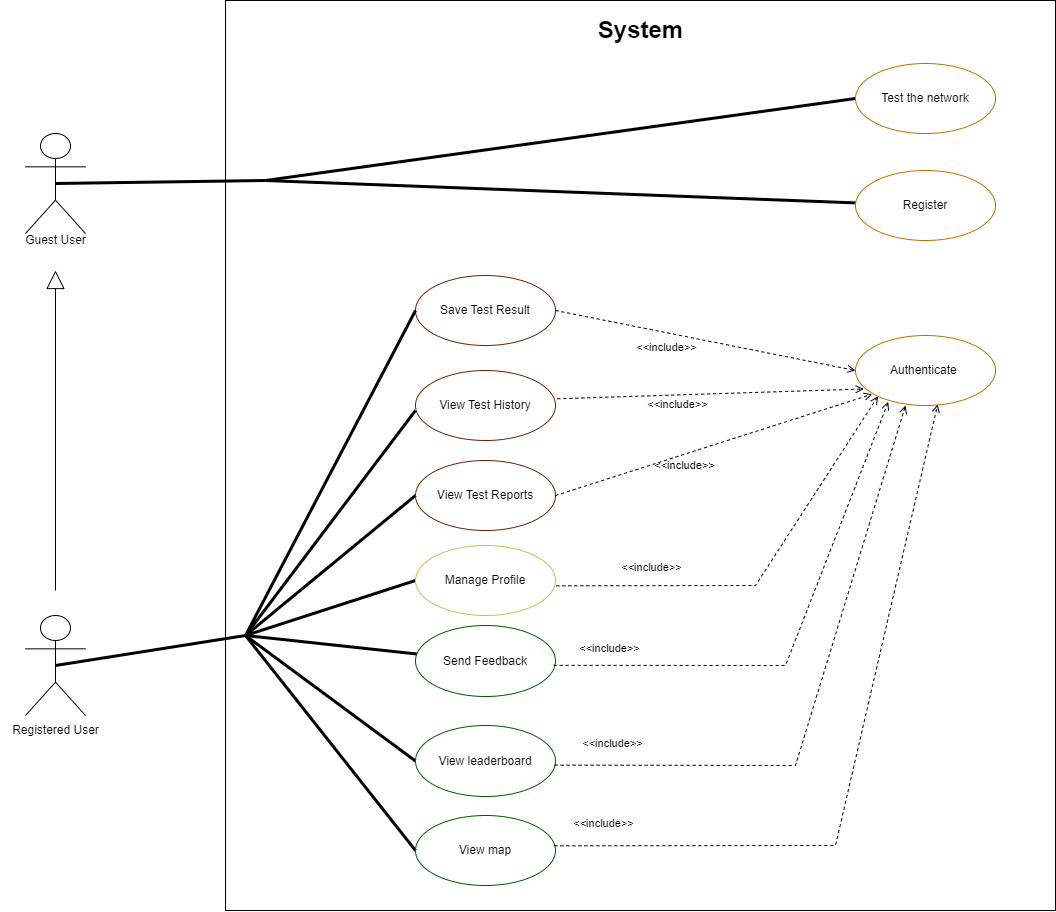
\includegraphics[width=1\textwidth]{images/chap1/gloabalUC.png}
    \caption{Global Use Case Diagram}
    \label{fig:enter-label}
\end{figure}

\newpage

\subsection{General class diagram : }

The class diagram provides a visual representation ofthe static structure of a system, including the classes, their attributes, methods, and the relationships between them.This diagram will cover the global class diagram of our application.
% Not done yet
\begin{figure}[H]
    \centering
    \includegraphics[width=0.97\textwidth]{images/global-class.pngp}
    \caption{General class diagram - Not done yet}
    \label{fig:enter-label}
\end{figure}




\newpage

\section{Project management with Scrum}

\subsection{Scrum projection on our project}
By adopting SCRUM as a project management approach we need to define actors 
and provide a product backlog from specified requirements earlier 
\subsubsection{Scrum actors in our team}

\begin{table}[H]
    \centering
    \begin{tabular}{|p{5cm}|p{5cm}|p{6.5cm}|}
    \hline
    \textbf{Member} & \textbf{Role} & \textbf{Task} \\ \hline
    \begin{center}
        \textbf{Bilel Othmen}
    \end{center} & \begin{itemize}
        \item Product Owner
    \end{itemize} & \begin{itemize}
        \item Identification of requirements and functionalities to be implemented
    \end{itemize} \\ \hline

    \begin{center}
        \textbf{Nizar Ben Soltane}
    \end{center} & \begin{itemize}
        \item Scrum Master
    \end{itemize} & \begin{itemize}
        \item Project Validation
    \end{itemize} \\ \hline

    \begin{center}
        \textbf{Hammami Mohamed Yacin}
    \end{center} & \begin{itemize}
        \item Development Team
    \end{itemize} & \begin{itemize}
        \item Development
        \item Validation and Testing
        \item Deployment
    \end{itemize} \\ \hline
    \end{tabular}
    \caption{SCRUM Actors}
    \label{tab:my_label}
    \setlength{\abovecaptionskip}{0.25cm}
\end{table}

\newpage


\subsection{Product Backlog}
From the requirements specified  earlier and the global use case diagram , we can extract a product backlog to be our guide in through this project 


\begin{table}[H]
% \begin{tabular}{|p{5cm}|p{5cm}|p{6.5cm}|}
\begin{tabular}{|p{0.5cm}|p{3cm}|p{7cm}|p{2cm}|p{2cm}|}
\hline
ID & Epic           & Description                                                               & Priority & Complexity \\ \hline
1  & Configuration & Administrator can specify the desired parameter that  the application will work with  & High     & basic      \\ \hline
2  & Authentication & User can authenticate to the app through a robust authentication system   & High     & basic      \\ \hline
3  & Network Test     & User can test his network, see results and save them                      & High     & medium     \\ \hline
4  & Cartography    & User can inspect the network state in his country in specific time period & High     & High       \\ \hline
5  & Reporting      & User can see detailed reports based on his tests                          & medium   & medium     \\ \hline
6  & Feedback       & User can send feedback or report issues to authorities                    & Low      & basic      \\ \hline
\end{tabular}
\caption{Product Backlog}
\label{tab:backlog}
\end{table}


\newpage

\section{Sprint Planning}

The 2.4 table illustrates the distribution of sprints and the duration of each one

\begin{table}[H]
    % \centering
    \renewcommand{\arraystretch}{1.5}
   
   \begin{tabular}{|p{0.15\textwidth}|p{0.61\textwidth}|p{0.15\textwidth}|}
   \hline
   \centering
   \textbf{Sprints } &  \textbf{Sprint Functionality} &\textbf{Duration}
\\ \hline
        \centering
       \textbf{Sprint 1}  &  
       \begin{itemize}[left=0pt,label={\textbf{-}}]
           \item Configurable application
           \item Navigation system
           \item Authentication system
       \end{itemize}
       & 
       \begin{itemize}[left=0pt,label={\textbf{-}}]
           \item  5 days
           \item  5 days
           \item  10 days
       \end{itemize}
       \\ \hline

       \centering
       \textbf{Sprint 2}  &  
       \begin{itemize}[left=0pt,label={\textbf{-}}]
           \item Map
           \item Leader-board 
       \end{itemize}
       &  \begin{itemize}[left=0pt,label={\textbf{-}}]
           \item  15 days
           \item  15 days
        
       \end{itemize} \\ \hline
       \centering
       \textbf{Sprint 3}  &  
       \begin{itemize}[left=0pt,label={\textbf{-}}]
           \item Network testing
           \item Report generation
       \end{itemize}
       &  \begin{itemize}[left=0pt,label={\textbf{-}}]
           \item  15 days
           \item  15 days
        
       \end{itemize} \\ \hline
       \centering
       \textbf{Sprint 4}  &  
       \begin{itemize}[left=0pt,label={\textbf{-}}]
           \item Feedback and reviews
       \end{itemize}
       &  \begin{itemize}[left=0pt,label={\textbf{-}}]
           \item  10 days
       \end{itemize} \\ \hline

       
       
\end{tabular}
     \caption{Sprint Planning Table}
    \label{tab:my_label}
     \setlength{\abovecaptionskip}{0.25cm}
\end{table}


\section{Working environment}

In this section, we provide details about the hardware and software environments that have been provided for our project.


\subsection{Hardware environment }
The technical specifications of the devices used are listed in the following table : 
\vspace{0.25cm}
\newpage
\begin{large}
    \textbf{Computer specifications}
\end{large}
\vspace{0.25cm}

\begin{table}[H]
    % \centering
    \renewcommand{\arraystretch}{1.5}
   \begin{tabular}{|p{0.3\textwidth}|p{0.61\textwidth}|}
   \hline
    
       \textbf{Computer} & Lenovo IdeaPad3 \\ \hline
       \textbf{Processor} & i5-10210U  \\ \hline
       \textbf{RAM} & 20 \\ \hline
       \textbf{Hard disk} & 512 SSD \\ \hline
       \textbf{Graphic card} & MX130  \\ \hline
       \textbf{Operating System} &Windows 10 Pro \\ \hline

\end{tabular}
     \caption{Computer specifications Table}
    \label{tab:my_label}
    % \setlength{\abovecaptionskip}{0.25cm}
\end{table}

\begin{large}
    \textbf{Smartphones specifications}
\end{large}

\begin{table}[H]
    % \centering
    \renewcommand{\arraystretch}{1.5}
    \setlength{\belowcaptionskip}{0.25cm}
    

   \begin{tabular}{|p{0.3\textwidth}|p{0.61\textwidth}|}
   \hline
    
       \textbf{Model name} & Samsung Galaxy A04 \\ \hline
       \textbf{OS} & Android 13\\ \hline
       \textbf{RAM} & 4 Gb \\ \hline
       \textbf{Battery} &  5000 mAh \\ \hline
       \textbf{Storage} & 64 Gb \\ \hline

\end{tabular}
   
    % \setlength{\abovecaptionskip}{0.25cm}
    \caption{Smartphones specifications Table}
    \label{tab:my_label}
\end{table}

\section{Software kit}
In recognition of its importance to the project's accomplishment, we'll be specifying the software  kit  used in this journey.  This information will also be helpful for anyone with questions about the project's technology stack.
\subsection{Project Management}
\subsection*{Jira}
For tracking our project and letting all team members to  have an updated vision on its progress we used Jira as Project management tool .
Jira Software is the \#1 agile project management tool used by teams to plan, track, release and support world-class software with confidence. It is the single source of truth for your entire development lifecycle, empowering autonomous teams with the context to move quickly while staying connected to the greater business goal. Whether used to manage simple projects or to power your DevOps practices, Jira Software makes it easy for teams to move work forward, stay aligned, and communicate in context.\cite{Jira}
% \cite{https://www.atlassian.com/software/jira/guides/getting-started/introduction}
\begin{figure}[H]
    \centering
    
\includegraphics[height=4cm]{images/chap1/jira.png}
    \caption{Jira Logo}
    \label{fig:enter-label}
\end{figure}
\subsection{Version Controle}
\subsection*{GitLab}
We used GitLab to store our application code and to facilitate integration in a CI/CD pipeline .
GitLab is an Open Source code repository and collaborative software development platform for large DevOps and DevSecOps projects. GitLab is free for individuals.

GitLab offers a location for online code storage and capabilities for issue tracking and CI/CD. The repository enables hosting different development chains and versions.\cite{GitLab}
% \cite{https://www.techtarget.com/whatis/definition/GitLab}
\begin{figure}[H]
    \centering
    
\includegraphics[height=4cm]{images/chap1/gitlab.png}
    \caption{GitLab Logo}
    \label{fig:enter-label}
\end{figure}

\subsection{Modeling}
\subsection*{Drawio}
We used Drawio to draw all diagrams used in this report,
draw.io is a technology stack for building diagramming applications, and the world’s most widely used browser-based end-user diagramming software. \cite{Drawio}
% \cite{https://www.drawio.com/about}
\begin{figure}[H]
    \centering
    
\includegraphics[height=4cm]{images/chap1/drawio.png}
    \caption{Drawio Logo}
    \label{fig:enter-label}
\end{figure}
% \subsection{Report Writing}
% \subsection*{LaTex}
% LaTeX is widely used in academia for the communication and publication of scientific documents and technical note-taking in many fields. It also has a prominent role in the preparation and publication of books and articles that contain complex multilingual materials, such as Arabic and Greek.LaTeX uses the TeX typesetting program for formatting its output, and is itself written in the TeX macro language.
% % \cite{https://en.wikipedia.org/wiki/LaTeX}
% \begin{figure}[H]
%     \centering
%     
\includegraphics[height=4cm]{images/chap1/Latex-logo.png}
%     \caption{LaTex Logo}
%     \label{fig:enter-label}
% \end{figure}
% \subsection*{Overleaf}
% Overleaf’s market-leading collaboration technology is now in use by over 15 million researchers, students, and teachers in institutions, labs, and industry worldwide.
% % \cite{https://www.overleaf.com/about}
% \begin{figure}[H]
%     \centering
%     
\includegraphics[height=4cm]{images/chap1/overleaf_wide_colour_light_bg.png}
%     \caption{Overleaf Logo}
%     \label{fig:enter-label}
% \end{figure}
\subsection{Development}
\subsubsection{Programming Language and Database}
\subsubsection*{Spring Boot}
As a robust backend we chose springboot as backend framework .
Java Spring Boot is an open-source tool that makes it easier to use Java-based frameworks to create microservices and web apps.\cite{Springboot} 
% \cite{https://azure.microsoft.com/en-us/resources/cloud-computing-dictionary/what-is-java-spring-boot}
\begin{figure}[H]
    \centering
    
\includegraphics[height=6cm]{images/chap1/springJava.png}
    \caption{Springboot \& Java Logo}
    \label{fig:enter-label}
\end{figure}
\subsubsection*{React Native}
To have a modern and complex UI , and to have a cross platform application , we adopted React-Native, 
React Native is an open-source UI software framework created by Meta Platforms, Inc. It is used to develop applications for Android: Android TV,iOS:, macOS, tvOS,Web, Windows and UWP by enabling developers to use the React framework along with native platform capabilities.\cite{ReactNative}
% \cite{https://en.wikipedia.org/wiki/React_Native}
\begin{figure}[H]
    \centering
    
\includegraphics[height=6cm]{images/chap1/reactnativeJS.png}
    \caption{React native \& Javascript Logo}
    \label{fig:enter-label}
\end{figure}
\subsubsection*{Expo}
To have a better developer experience building this application , we used Expo to benefit its outstanding features .
Expo is a set of tools and services built around React Native and, while it has many features, the most relevant feature for us right now is that it can get you writing a React Native app within minutes. You will only need a recent version of Node.js and a phone or emulator. \cite{Expo}
% \cite{https://reactnative.dev/docs/environment-setup#:~:text=Expo%20is%20a%20set%20of,and%20a%20phone%20or%20emulator.}
\begin{figure}[H]
    \centering
    
\includegraphics[height=6cm]{images/chap1/expo.png}
    \caption{Expo Logo}
    \label{fig:enter-label}
\end{figure}

\subsubsection*{PostgreSQL}
To store all application's data , our decision was PostgreSQL as a RDBMS. 
PostgreSQL is an advanced, enterprise-class, and open-source relational database system. PostgreSQL supports both SQL (relational) and JSON (non-relational) querying.\cite{PostgreSQL}
% \cite{https://www.postgresqltutorial.com/postgresql-getting-started/what-is-postgresql/}
\begin{figure}[H]
    \centering
    
\includegraphics[height=4cm]{images/chap1/postgres.png}
    \caption{PostgreSQL Logo}
    \label{fig:enter-label}
\end{figure}



\subsection{Code Editor}
\subsubsection*{VsCode}
To write code , test it and push it to GitLab ,VsCode was a great tool for providing that and more features to facilitate the development journey .
Visual Studio Code is a free coding editor that helps you start coding quickly. Use it to code in any programming language, without switching editors. Visual Studio Code has support for many languages.\cite{VSCode}
% \cite{https://code.visualstudio.com/learn}
\begin{figure}[H]
    \centering
    
\includegraphics[height=4cm]{images/chap1/vscode.jpg}
    \caption{Vscode Logo}
    \label{fig:enter-label}
\end{figure}
\subsection{Testing}
\subsubsection*{Postman}
To test our API endpoints , we used Postman .
Postman is an API platform for building and using APIs. Postman simplifies each step of the API lifecycle and streamlines collaboration so you can create better APIs—faster.\cite{Postman}
% \cite{https://www.postman.com/product/what-is-postman/}
\begin{figure}[H]
    \centering
    
\includegraphics[height=4cm]{images/chap1/postman.jpg}
    \caption{Postman Logo}
    \label{fig:enter-label}
\end{figure}





\subsection{Application's Architecture}
The structure of an application, known as application architecture encompasses its core design elements, including components, their connections and the guiding design principles. It covers aspects such, as;
\begin{enumerate}
    \item  \underline{\textbf{Component Arrangement}:}
 This involves identifying the parts or sections of the application. How they interact with each other. Components can range from user interfaces to databases, services, APIs and external systems.

\item  \underline{\textbf{Data Handling}:} How information is stored, retrieved, updated and managed within the application. This includes selecting databases, data models and storage methods.

\item  \underline{\textbf{Communication Methods}:} Specifies how different components communicate with each other. This could involve asynchronous communication using protocols, like HTTP, WebSockets or message queues.

\item  \underline{Handling Concurrency and Scalability:} How the application manages users concurrently. Expands to handle increased loads. Considerations include managing threads load distribution strategies and horizontal expansion.
\end{enumerate}
\subsubsection{MVC Architecture}
In this project we adopted the Model-View-Controller Architecture known as MVC ,to have an enhanced code organization, and to facilitate maintenance and scalability , in fact separate the application's logic into distinct layers, each of which holds a specific set of tasks as follow :
\begin{itemize}
    \item \textbf{Model:} The layer that manages the applications data operations is responsible, for tasks like storing and retrieving data from databases. It also includes features for validating data and performing data related functions. Its main role is to maintain the integrity and accessibility of all data aspects.

    \item \textbf{View: }The layer that showcases the user interface needed for interacting with the application consists of components for displaying data and enabling user interaction. This may include elements such as buttons, links, tables, dropdown menus or input fields.

    \item \textbf{Controller: }The layer that coordinates the applications logic facilitates communication, between the view and model layers. Regarded as the engine of the application it oversees the flow and synchronization of operations.

\end{itemize}
\begin{figure}[H]
    \centering
    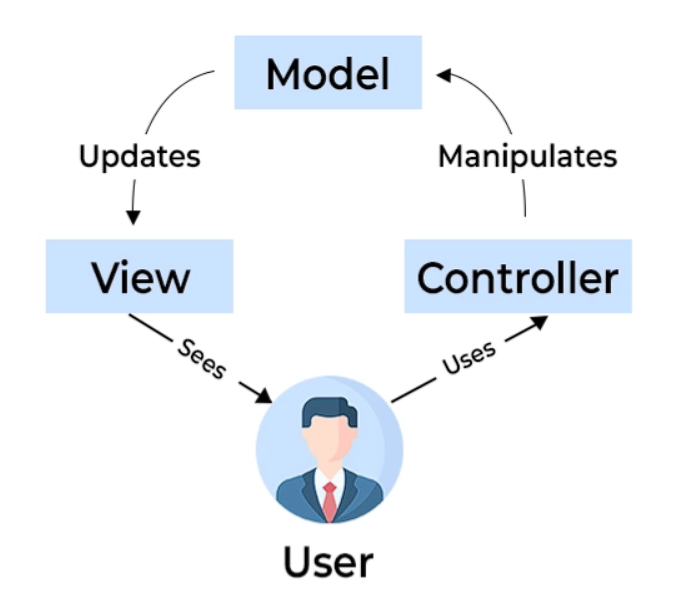
\includegraphics[height=7cm]{images/chap1/mvc.png}
    \caption{MVC architecture}
    \label{fig:enter-label}
\end{figure}






\section*{Conclusion}

During this chapter, we identified the functional and non-functional requirements of the system, as well as the main actors and their roles. Afterwards, we identified the product backlog and sprint planning. We concluded the chapter by explaining the architecture of our application. In the next chapter, we will begin the development of Sprint 1.
